% lec6s20.m4: Netzwerk fuer Kontenpotentialverfahren nach Kasper
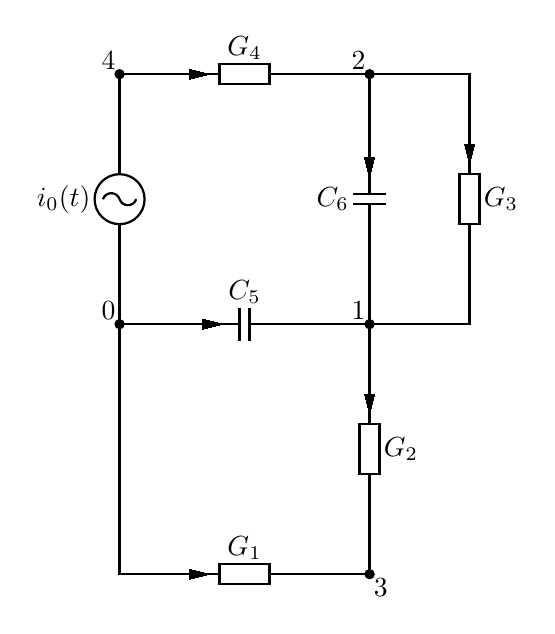
\begin{tikzpicture}[scale=2.54]%
% dpic version 2024.01.01 option -g for TikZ and PGF 1.01
\ifx\dpiclw\undefined\newdimen\dpiclw\fi
\global\def\dpicdraw{\draw[line width=\dpiclw]}
\global\def\dpicstop{;}
\dpiclw=0.8bp
\dpiclw=0.8bp
\dpicdraw[fill=black](0,0) circle (0.007874in)\dpicstop
\draw (0,0) node[above left=-2bp]{0};
\dpicdraw (0,0)
 --(0.25,0)\dpicstop
\dpicdraw (0.25,0)
 --(0.6,0)\dpicstop
\dpicdraw (0.6,-0.083333)
 --(0.6,0.083333)\dpicstop
\dpicdraw (0.65,-0.083333)
 --(0.65,0.083333)\dpicstop
\dpicdraw (0.65,0)
 --(1,0)\dpicstop
\draw (0.625,0.083333) node[above=-2bp]{$ C_5$};
\filldraw[line width=0bp](0.416667,-0.025)
 --(0.516667,0)
 --(0.416667,0.025) --cycle\dpicstop
\dpicdraw (0.493761,0)
 --(0.416667,0)\dpicstop
\dpicdraw (1,0)
 --(1.25,0)\dpicstop
\dpicdraw[fill=black](1.25,0) circle (0.007874in)\dpicstop
\draw (1.25,0) node[above left=-2bp]{1};
\dpicdraw (1.25,0)
 --(1.25,-0.25)\dpicstop
\dpicdraw (1.25,-0.25)
 --(1.25,-0.5)\dpicstop
\dpicdraw (1.25,-0.75)
 --(1.3,-0.75)
 --(1.3,-0.5)
 --(1.2,-0.5)
 --(1.2,-0.75)
 --(1.25,-0.75)\dpicstop
\dpicdraw (1.25,-0.75)
 --(1.25,-1)\dpicstop
\draw (1.3,-0.625) node[right=-2bp]{$ G_2$};
\filldraw[line width=0bp](1.225,-0.35)
 --(1.25,-0.45)
 --(1.275,-0.35) --cycle\dpicstop
\dpicdraw (1.25,-0.427094)
 --(1.25,-0.35)\dpicstop
\dpicdraw (1.25,-1)
 --(1.25,-1.25)\dpicstop
\dpicdraw[fill=black](1.25,-1.25) circle (0.007874in)\dpicstop
\draw (1.25,-1.25) node[below right=-2bp]{3};
\dpicdraw (1.25,-1.25)
 --(1,-1.25)\dpicstop
\dpicdraw (1,-1.25)
 --(0.75,-1.25)\dpicstop
\dpicdraw (0.5,-1.25)
 --(0.5,-1.3)
 --(0.75,-1.3)
 --(0.75,-1.2)
 --(0.5,-1.2)
 --(0.5,-1.25)\dpicstop
\dpicdraw (0.5,-1.25)
 --(0.25,-1.25)\dpicstop
\draw (0.625,-1.2) node[above=-2bp]{$ G_1$};
\filldraw[line width=0bp](0.35,-1.275)
 --(0.45,-1.25)
 --(0.35,-1.225) --cycle\dpicstop
\dpicdraw (0.427094,-1.25)
 --(0.35,-1.25)\dpicstop
\dpicdraw (0.25,-1.25)
 --(-0,-1.25)
 --(0,0)\dpicstop
\dpicdraw (0,0)
 --(0,0.25)\dpicstop
\dpicdraw (0,0.25)
 --(0,0.5)\dpicstop
\dpicdraw (0,0.625) circle (0.049213in)\dpicstop
\dpicdraw (-0,0.625)
 ..controls (-0.005978,0.642935) and (-0.022762,0.655032)
 ..(-0.041667,0.655032)
 ..controls (-0.060571,0.655032) and (-0.077355,0.642935)
 ..(-0.083333,0.625)\dpicstop
\dpicdraw (0,0.625)
 ..controls (0.005978,0.607065) and (0.022762,0.594968)
 ..(0.041667,0.594968)
 ..controls (0.060571,0.594968) and (0.077355,0.607065)
 ..(0.083333,0.625)\dpicstop
\dpicdraw (0,0.75)
 --(0,1)\dpicstop
\draw (-0.125,0.625) node[left=-2bp]{$ i_0(t)$};
\dpicdraw (0,1)
 --(0,1.25)\dpicstop
\dpicdraw[fill=black](0,1.25) circle (0.007874in)\dpicstop
\draw (0,1.25) node[above left=-2bp]{4};
\dpicdraw (0,1.25)
 --(0.25,1.25)\dpicstop
\dpicdraw (0.25,1.25)
 --(0.5,1.25)\dpicstop
\dpicdraw (0.75,1.25)
 --(0.75,1.3)
 --(0.5,1.3)
 --(0.5,1.2)
 --(0.75,1.2)
 --(0.75,1.25)\dpicstop
\dpicdraw (0.75,1.25)
 --(1,1.25)\dpicstop
\draw (0.625,1.3) node[above=-2bp]{$ G_4$};
\filldraw[line width=0bp](0.35,1.225)
 --(0.45,1.25)
 --(0.35,1.275) --cycle\dpicstop
\dpicdraw (0.427094,1.25)
 --(0.35,1.25)\dpicstop
\dpicdraw (1,1.25)
 --(1.25,1.25)\dpicstop
\dpicdraw[fill=black](1.25,1.25) circle (0.007874in)\dpicstop
\draw (1.25,1.25) node[above left=-2bp]{2};
\dpicdraw (1.25,1.25)
 --(1.75,1.25)
 --(1.75,1)\dpicstop
\dpicdraw (1.75,1)
 --(1.75,0.75)\dpicstop
\dpicdraw (1.75,0.5)
 --(1.8,0.5)
 --(1.8,0.75)
 --(1.7,0.75)
 --(1.7,0.5)
 --(1.75,0.5)\dpicstop
\dpicdraw (1.75,0.5)
 --(1.75,0.25)\dpicstop
\draw (1.8,0.625) node[right=-2bp]{$ G_3$};
\filldraw[line width=0bp](1.725,0.9)
 --(1.75,0.8)
 --(1.775,0.9) --cycle\dpicstop
\dpicdraw (1.75,0.822906)
 --(1.75,0.9)\dpicstop
\dpicdraw (1.75,0.25)
 --(1.75,-0)
 --(1.25,0)\dpicstop
\dpicdraw (1.25,1.25)
 --(1.25,1)\dpicstop
\dpicdraw (1.25,1)
 --(1.25,0.65)\dpicstop
\dpicdraw (1.166667,0.65)
 --(1.333333,0.65)\dpicstop
\dpicdraw (1.166667,0.6)
 --(1.333333,0.6)\dpicstop
\dpicdraw (1.25,0.6)
 --(1.25,0.25)\dpicstop
\draw (1.166667,0.625) node[left=-2bp]{$ C_6$};
\filldraw[line width=0bp](1.225,0.833333)
 --(1.25,0.733333)
 --(1.275,0.833333) --cycle\dpicstop
\dpicdraw (1.25,0.756239)
 --(1.25,0.833333)\dpicstop
\dpicdraw (1.25,0.25)
 --(1.25,0)\dpicstop
\end{tikzpicture}%
